\section{Pythagoras as a law of accounting}
\label{sec:pythagoras}

The Pythagorean theorem is usually presented as a fact about Euclidean triangles.
From the accounting point of view it is a statement about costs: if the cost of a displacement is a positive quadratic form, and the two coordinate directions are orthogonal for that form, then the cost of a diagonal displacement is the sum of the costs of its two legs.
This section shows that staging an isotropic walk produces exactly this situation, with uniform error bounds, and that a matched walk with correlated steps produces a quadratic cost for which the coordinate axes are not orthogonal.

The setting differs from that of \cref{sec:constructed}.
There is no lens: we consider the one-shot cost of a long displacement, not the cheapest chain of macro transitions.
Let $p_n(z)$ be the probability that the lazy walk on $\Z^2$ (stay with probability $\tfrac12$, each cardinal move with probability $\tfrac18$) is displaced by $z$ after $n$ steps.
The \emph{staged cost} is $-\log p_n(z)$, and the \emph{centred cost} is $F_n(z)=\log\bigl(p_n(0)/p_n(z)\bigr)$.

\subsection{A uniform quadratic limit}

\begin{theorem}[Uniform local estimate]
\label{thm:local-limit}
Let $g_n(z)=\frac{2}{\pi n}\exp(-2|z|^2/n)$ and $a=11/96$.
For every $n\ge2$ and every $z\in\Z^2$,
\begin{equation}
|p_n(z)-g_n(z)|\;\le\;B_n\coloneqq\frac{7}{768\pi a^3}\,\frac{n}{(n-1)^3}+\frac{\pi}{2n}e^{-n/(2\pi^2)}+\frac{2}{\pi n}e^{-n/8}.
\end{equation}
\end{theorem}

\provenance{Written proof (\cref{app:quadratic-proof}) from the exact Fourier inversion formula for $p_n$, whose characteristic function $\varphi(t)=\tfrac12+\tfrac14(\cos t_1+\cos t_2)$ takes values in $[0,1]$, together with elementary Taylor and sine bounds and an explicit Gaussian integral. No weak-convergence argument is used.}

The coefficient $2/n$ is not fitted: it is the inverse of twice the per-axis variance $n/4$ of the walk.
Dividing by the explicit lower bound on $g_n$ in a central window gives a relative error, which is what is needed before taking logarithms.

\begin{corollary}[Quadratic accounting and a Euclidean readout]
\label{cor:quadratic}
Fix $R\ge0$ and put
\begin{equation}
E_R(n)=e^{2R^2}\Bigl[\tfrac{4032}{1331}\,\tfrac{n^2}{(n-1)^3}+\tfrac{\pi^2}{4}e^{-n/(2\pi^2)}+e^{-n/8}\Bigr],\qquad d_R(n)=\frac{2E_R(n)}{1-E_R(n)}.
\end{equation}
Whenever $E_R(n)<1$, every $z$ with $|z|\le R\sqrt n$ has $p_n(z)>0$ and $F_n(z)\ge0$, and
\begin{align}
\bigl|F_n(z)-2|z|^2/n\bigr|&\le d_R(n), \label{eq:quad-limit}\\
\bigl|-\log p_n(z)-\log(\pi n/2)-2|z|^2/n\bigr|&\le \frac{E_R(n)}{1-E_R(n)},\\
\bigl|F_n(x,y)-F_n(x,0)-F_n(0,y)\bigr|&\le3\,d_R(n), \label{eq:axis-residual}\\
\Bigl|\sqrt{F_n(z)/2}-|z|/\sqrt n\Bigr|&\le\sqrt{d_R(n)/2}. \label{eq:readout}
\end{align}
Since $E_R(n)=O_R(1/n)$, all four errors tend to zero uniformly on the window.
\end{corollary}

\provenance{Written proof from \cref{thm:local-limit}. Nonnegativity of $F_n$ follows from $p_n(0)-p_n(z)=(2\pi)^{-2}\int\varphi^n(1-\cos t\cdot z)\,dt\ge0$, which uses $\varphi\ge0$. Lean: \lean{abs_log_le_relative_error}, \lean{log_cost_error}, \lean{centered_log_ratio_error}, \lean{cost_axis_residual_bound} (\lean{QuadraticLimit.lean}) and \lean{quadratic_cost_readout_error} (\lean{Pythagoras.lean}) mechanize the passage from relative probability error to the cost, residual and readout bounds.}

Three consequences are worth spelling out.
First, \eqref{eq:quad-limit} says that the staged cost becomes a quadratic form in the displacement, with offset $\log(\pi n/2)$ and coefficient $2/n$ both predicted from the dynamics.
Second, \eqref{eq:axis-residual} says that the cost of a diagonal displacement equals the sum of the costs of its legs, up to a vanishing error: this is the Pythagorean law in cost form.
Third, \eqref{eq:readout} gives a genuine Euclidean geometry.
Let $K$ be a bounded set in the plane, represent $u\in K$ on the lattice by $z_n(u)=(\lfloor\sqrt n\,u_1\rfloor,\lfloor\sqrt n\,u_2\rfloor)$, and choose $R\ge\operatorname{diam}(K)+\sqrt2$, so that every difference $z_n(u)-z_n(v)$ lies in the window $|z|\le R\sqrt n$. Whenever $E_R(n)<1$,
\begin{equation}
\sup_{u,v\in K}\Bigl|\sqrt{F_n\bigl(z_n(u)-z_n(v)\bigr)/2}-|u-v|\Bigr|\;\le\;\sqrt{d_R(n)/2}+\sqrt{2/n}\;\longrightarrow\;0,
\end{equation}
so the square-root readout of the staged cost converges uniformly to Euclidean distance.
The squared cost itself is not a metric (squared distance violates the triangle inequality on the points $0,1,2$ of a line), and the finite readout need not satisfy the triangle inequality exactly; its limit does.

\paragraph{Finite substrates.}
On a torus of side $N$, displacements up to $n$ steps cannot wrap around onto other reachable displacements when $N>2n$, so the torus probabilities coincide with the lattice ones.
This covers the torus of side $512$ used below for all stages up to $128$.
An asymptotic statement on tori requires $N$ to grow with $n$; on a fixed torus the walk eventually becomes uniform and the quadratic law disappears.
For the same reason the theorem uses the true probabilities: a fixed positive probability floor or fitting threshold would eventually discard central probabilities, which are of order $1/n$.

\subsection{Exact certificates and finite runs}

The bounds of \cref{cor:quadratic} are conservative; at the original stages an exact certificate is sharper.
The probabilities are $\mathrm{count}_\tau(z)/8^\tau$ with integer counts computed by exact recurrence. For the six stages $\tau=4,8,16,32,64,128$, on the windows $|x|,|y|\le\lfloor\sqrt\tau\rfloor$, the inequality $|F_\tau(z)-2|z|^2/\tau|\le\delta_\tau$ is verified using rational enclosures of the exponential function.
The certified errors are $\delta_\tau=\tfrac{363}{500},\tfrac{117}{1000},\tfrac{177}{1000},\tfrac{11}{200},\tfrac{11}{250},\tfrac1{50}$ for $\tau=4,8,16,32,64,128$ (windows of $25$ to $529$ points; \cref{fig:quadratic}d).
At $\tau=128$ the readout $\sqrt{F_\tau/2}$ is therefore within $\sqrt{\delta_\tau/2}=0.1$ of $|z|/\sqrt\tau$ on the whole $529$-point window.

\provenance{Exact computation (integer recurrence and rational Taylor enclosures of degree $80$, rebuilt by an independent verifier). Lean: \lean{quadratic_cost_readout_error} turns the certified bound into the readout bound.}

\begin{figure}[t]
\centering
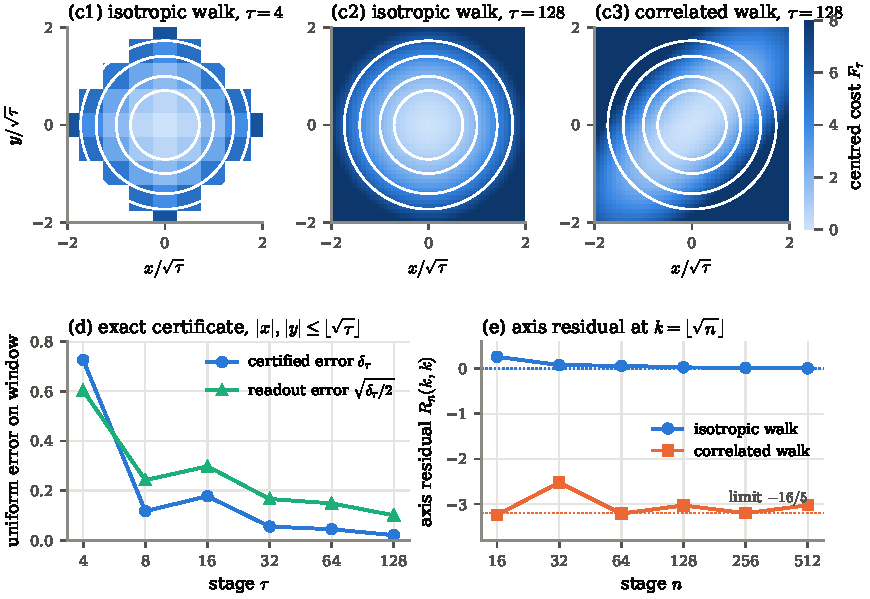
\includegraphics[width=\linewidth]{figures/fig_quadratic.pdf}
\caption{Quadratic accounting. (c1--c3) Centred cost $F_\tau$ in diffusive units $z/\sqrt\tau$; white circles are the level sets $2|z|^2/\tau\in\{1,2,4,6\}$ of the isotropic limit, blank cells are unreachable displacements. At $\tau=4$ the support is a diamond; at $\tau=128$ the isotropic cost is approximately circular, while the correlated walk's cost is approximately elliptical with axes along the diagonals. (d) Exact certificate: uniform centred-cost error $\delta_\tau$ and readout error $\sqrt{\delta_\tau/2}$ on the windows $|x|,|y|\le\lfloor\sqrt\tau\rfloor$. (e) Axis residual $F_n(k,k)-F_n(k,0)-F_n(0,k)$ at $k=\lfloor\sqrt n\rfloor$; the correlated walk's residual equals $-\tfrac{16}5k^2/n$ up to a vanishing error, which oscillates with the rounding of $\sqrt n$ and tends to $-16/5$. Panels (c) and (e): floating computation by nonnegative convolution; panel (d): exact.}
\label{fig:quadratic}
\end{figure}

Floating-point runs on the torus of side $512$ give a consistent picture over larger windows (half-width $\lceil3\sqrt\tau\,\rceil$, capped at $30$), with probabilities computed by nonnegative convolution so that unreachable displacements have probability exactly zero.
A least-squares quadratic fit to the cost has root-mean-square error $0.471$ at $\tau=4$ and $0.151$ at $\tau=128$ ($0.246$ and $0.024$ relative to the spread of the cost), and the median absolute axis residual over $2000$ sampled right triangles drops from $0.862$ to $0.059$.
Neither trend is monotone: as the window grows with $\tau$ the fit error first rises, to $1.19$ at $\tau=32$, before falling.
At $\tau=4$ only $307$ of the $2000$ triangles are supported, so these comparisons are over changing domains and are descriptive only.
Along the axes, a quadratic model fits the cost with error $0.018$ at $\tau=128$, against $1.05$ for a linear model.

\subsection{Controls}

\paragraph{What the residual does and does not test.}
The axis residual~\eqref{eq:axis-residual} tests \emph{separability} of the cost along the coordinate axes, not quadratic shape.
The Manhattan cost $|x|+|y|$ has residual exactly zero, yet its contours are diamonds, its axis profile is linear, and squaring it violates the Pythagorean identity by $2|xy|$.
Quadratic shape is established separately, by~\eqref{eq:quad-limit}, by the certificate, and by the axis fits.

\paragraph{A matched dynamical control.}
Keep the holding probability $\tfrac12$, give each cardinal move probability $\tfrac1{16}$, and add the diagonal moves $(1,1)$ and $(-1,-1)$ with probability $\tfrac18$ each.
The step covariance becomes $\Sigma=\bigl(\begin{smallmatrix}3/8&1/4\\1/4&3/8\end{smallmatrix}\bigr)$, and the same Fourier argument gives a uniform local estimate with the limiting cost
\begin{equation}
Q_n(x,y)=\frac{z^{\mathsf T}\Sigma^{-1}z}{2n}=\frac{12}{5}\,\frac{x^2+y^2}{n}-\frac{16}{5}\,\frac{xy}{n}.
\end{equation}
The cross term makes the axis residual at the diagonal displacement $x=y=\lfloor\sqrt n\rfloor$ tend to $-16/5$ (\cref{fig:quadratic}e); exact certificates at $n=16,32,64,128$ place it strictly below $-1$.
The control does not destroy the Pythagorean law.
$Q_n$ is still a positive quadratic form, and Pythagoras holds for its own inner product; what fails is the orthogonality of the coordinate axes.
Correlation or anisotropy therefore changes \emph{which} directions are orthogonal, and an anisotropic walk with diagonal covariance would keep the coordinate axes orthogonal while turning circles into ellipses.

\provenance{Written proof (Fourier estimate for the correlated walk, \cref{app:quadratic-proof}). Exact computation: integer counts with denominator $16^n$ and rational logarithm enclosures at four stages. Floating computation: \cref{fig:quadratic}e.}

\paragraph{Relation to the macro metric.}
The staged cost is a one-shot account of a single long displacement.
It is not the shortest-path metric of \cref{sec:construction}, and comparing a diagonal cost with the sum of two axis costs at the same $\tau$ is an identity about the shape of the cost, not a statement that a $\tau$-step protocol costs the same as two composed $\tau$-step protocols.
The open-grid walk of \cref{sec:grid} follows the same bulk rule (hold with probability $\tfrac12$, otherwise move to a uniformly chosen neighbour) and differs only at the boundary, where the moving probability is shared among fewer neighbours; under block lenses its path metric converges to the $L^1$ distance.
Both geometries are legitimate readouts of the same local rule; they answer different accounting questions.
